\newpage
\hypertarget{initialize vis}{}
\subsection{Establishing the visual TGG}
\visHeader

\begin{itemize}

\item[$\blacktriangleright$] If you haven't already, double-click \texttt{Dict\-ion\-ary.eap} to open it in Enterprise Architect (EA). The project broswer
should resemble Fig.~\ref{ea:mocaTagged}. As you can see, the project is already populated with the source \texttt{MocaTree} specification for a generic tree structure.

\begin{figure}[htpb]
\begin{center}
  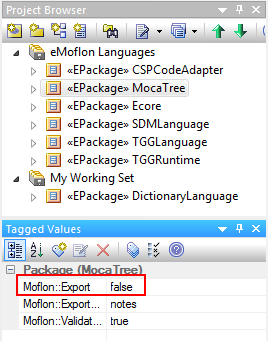
\includegraphics[width=0.4\textwidth]{ea_mocaTaggedValues}
  \caption{Preventing \texttt{MocaTree from exporting to Eclipse}}
  \label{ea:mocaTagged}
\end{center}
\end{figure}

\end{itemize}

If you inspect the tagged values\footnote{The ``Tagged Values'' window can be opened by going to ``View/Tagged Values''} for each language, you'll notice that
the \texttt{MocaTree} package has the \texttt{Moflon::Export} value set to \texttt{false}. This ensures that the package is \emph{ignored} when exporting. As
with all standard metamodels (e.g., Ecore or the SDM metamodel) the \texttt{MocaTree} package in EA should be regarded as read-only, required only in the
EA project so that SDMs can refer to the classes defined in the package. As discussed, the Java code is provided and added by our Eclipse plugin.

\begin{itemize}

\item[$\blacktriangleright$] Go ahead and inspect the \texttt{MocaTree} metamodel diagram (Fig.~\ref{ea:mocaTree}). Make sure you understand which attributes
each element contains and again, review it until you feel comfortable with what you'll be working with.

\item[$\blacktriangleright$] Given that TGGs can only succeed when the involved metamodels are contained in the same working set, add a new package to
\texttt{My Working Set} node named \texttt{Dict\-ion\-ary\-Code\-Adap\-ter}.

\newpage

\begin{figure}[htpb]
\begin{center}
  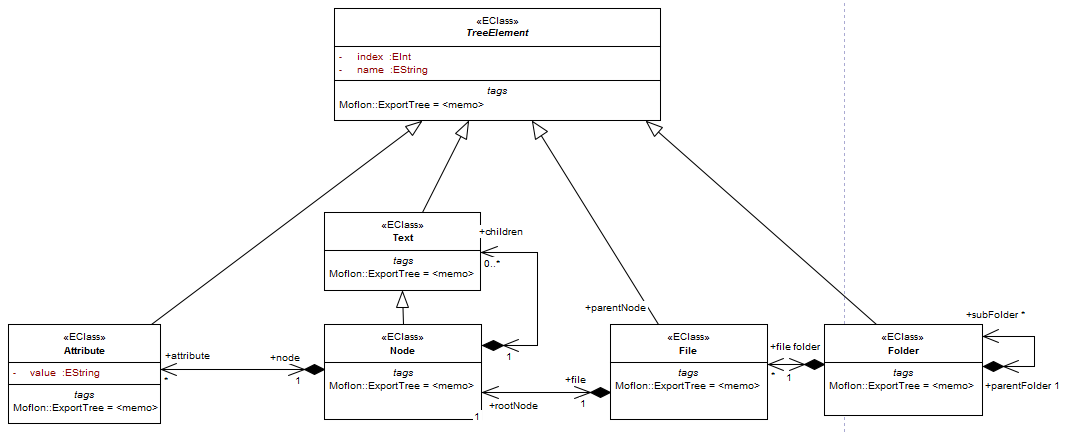
\includegraphics[width=\textwidth]{ea_metamodelMocaTree}
  \caption{The MocaTree Metamodel}
  \label{ea:mocaTree}
\end{center}
\end{figure}

\vspace{1cm}

\item[$\blacktriangleright$] Add a new TGG schema diagram as depicted in Fig.~\ref{ea:newTGGDiagram}. In the next dialogue that appears, set the source project
as \texttt{MocaTree}, and the target project as \texttt{Dict\-ion\-ary\-Lang\-uage}.

\vspace{1cm}

\begin{figure}[htpb]
\begin{center}
  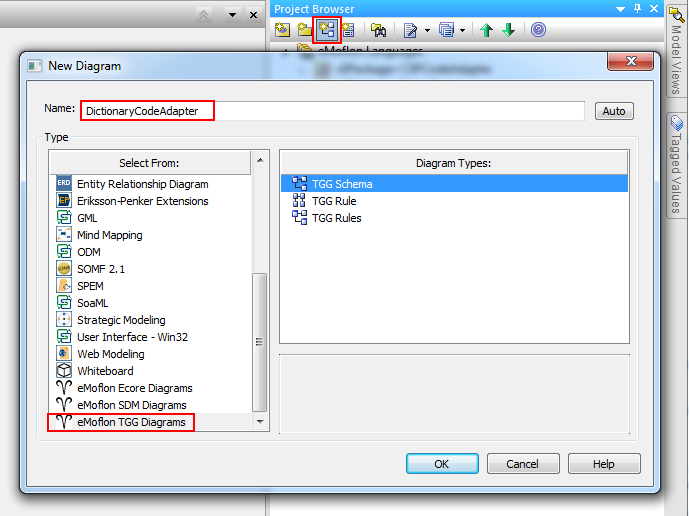
\includegraphics[width=0.85\textwidth]{ea_adapterTGGDiagram}
  \caption{Create a new TGG Diagram}
  \label{ea:newTGGDiagram}
\end{center}
\end{figure}

\end{itemize}

\clearpage

It should be mentioned that our conventions and workflow state that this \emph{code adapter} is a package that contains the tree-to-model transformation logic.
This could be integrated directly in the corresponding metamodel (\texttt{Dic\-tion\-ary\-Language}), but a separation makes sense here as there could be
\emph{different} code adapters for the \emph{same} language.

\begin{itemize}

\item[$\blacktriangleright$] To ensure the package exports correctly to the Eclipse workspace as a TGG project, add a single correspondence type to the
your diagram (the \texttt{schema}) between \texttt{Folder} and \texttt{Library}. You can do this by drag-and-dropping each element into the diagram,
then quick-linking a new TGG Correspondence type.\footnote{For details on how to do this, refer to Part IV, Section \update.} Your diagram should come to
resemble Fig.~\ref{ea:firstCorrType}.

\vspace{0.5cm}

\begin{figure}[htpb]
\begin{center}
  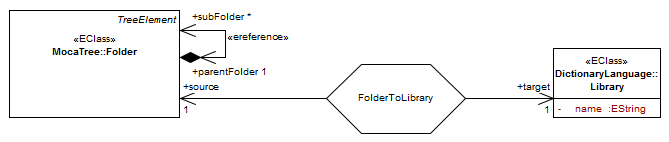
\includegraphics[width=\textwidth]{ea_firstAdapterCorrespondence}
  \caption{The transformation's first correspondence type}
  \label{ea:firstCorrType}
\end{center}
\end{figure}

\vspace{0.5cm}

\item[$\blacktriangleright$] Save and validate the project via the eMoflon control panel.\footnote{Introducted in Part \update, Section \update.} Switch back
to Eclipse and refresh the package explorer. A new \texttt{Dict\-ion\-ary\-Code\-Adap\-ter} folder should be generated for the TGG EPackage in \texttt{My
Working Set}; Your workspace is nearly complete!

\jumpSingle{subSec:setupParser}

\end{itemize}
